\documentclass{beamer}
\usepackage{graphicx}

\begin{document}

\begin{frame}{Proposed Zoning 1/15/2024}
    \begin{figure}[htb]
        \centering
        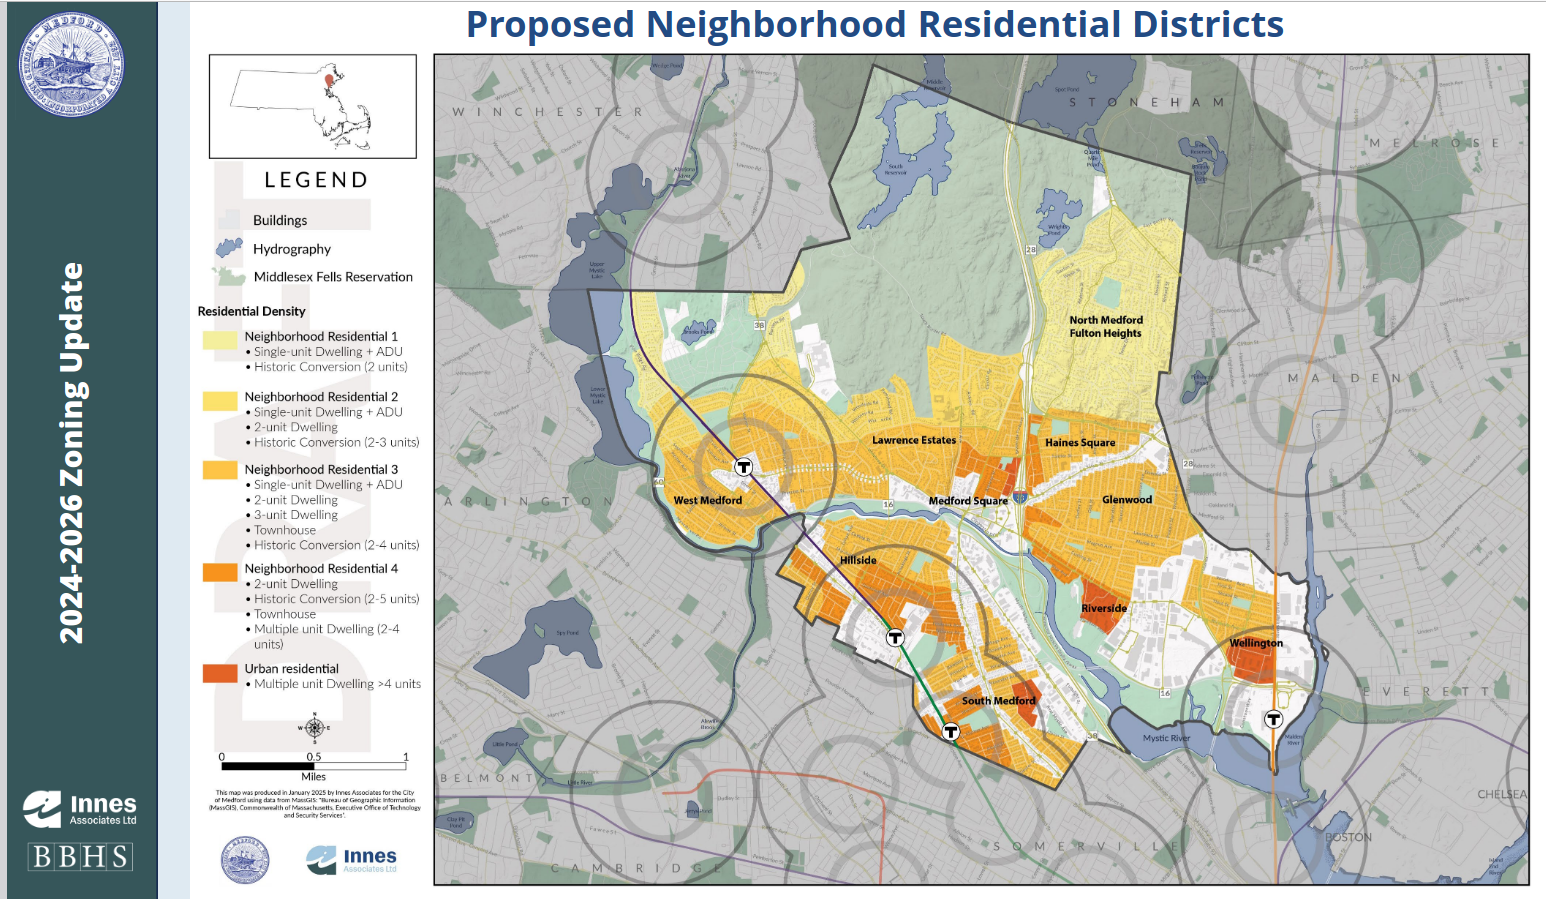
\includegraphics[width=0.8\textwidth,height=0.8\textheight,keepaspectratio]{resources/20240115/proposed_map.png}
    \end{figure}
\end{frame}

\begin{frame}{Adjust the Proposed Neighborhood Residential Districts by}
    \begin{itemize}
        \item Removint the NR-4 district type and consider it as part of the "urban residential" topic, potentially as an "urban residential 1" district.
        \item Classify all areas currently listed on the proposal as NR-1 or NR-2 as NR-1.
        \item Classify all areas currently listed on the proposal as NR-3 as NR-2.
        \item Classify all areas currently listed on the proposal as NR-4 as NR-3.
        \item Adjust the NR-3 district type to remove the 1-unit dwelling unit by-right.
        \item Any parcel where the current district is GR should be at least NR-2.
        \item Any parcel where the current district is APT-1 or APT-2 should be at least NR-3.
    \end{itemize}
\end{frame}

\begin{frame}{Discussion}
  \begin{itemize}
    \item Most deliberation on the amendment was focused on Lawrence Estate. Should duplexes be allowed there? 
    \item Fair to point out: Duplex \textit{plus} ADU was never on the table in Lawrence Estate.
    \item Is a single family home plus an ADU that different from a duplex?
    \item I don't really think that Lawrence Estate needs to be ``protected'' from duplexes, but I also don't think that this is a massive downsize from what the consultants proposed. So I am not \textit{that} concerned.
  \end{itemize}
\end{frame}

\begin{frame}{GT}
    \begin{figure}[htb]
        \centering
        \begin{tabular}{cc}
            \includegraphics[width=0.4\textwidth,height=0.4\textheight,keepaspectratio]{UNIT_GT_1.png} &
            \includegraphics[width=0.4\textwidth,height=0.4\textheight,keepaspectratio]{UNIT_GT_2.png} \\
            \includegraphics[width=0.4\textwidth,height=0.4\textheight,keepaspectratio]{UNIT_GT_4.png} &
            \includegraphics[width=0.4\textwidth,height=0.4\textheight,keepaspectratio]{UNIT_GT_8.png}
        \end{tabular}
    \end{figure}
\end{frame}

\begin{frame}{LT}
    \begin{figure}[htb]
        \centering
        \begin{tabular}{cc}
            \includegraphics[width=0.4\textwidth,height=0.4\textheight,keepaspectratio]{UNIT_LT_1.png} &
            \includegraphics[width=0.4\textwidth,height=0.4\textheight,keepaspectratio]{UNIT_LT_2.png} \\
            \includegraphics[width=0.4\textwidth,height=0.4\textheight,keepaspectratio]{UNIT_LT_4.png} &
            \includegraphics[width=0.4\textwidth,height=0.4\textheight,keepaspectratio]{UNIT_LT_8.png}
        \end{tabular}
    \end{figure}
\end{frame}

\begin{frame}{Magoun Area Triangle}
    \centering
    \includegraphics[width=0.6\textwidth,height=0.6\textheight,keepaspectratio]{magoun.png}
    \hspace{0.5cm}
    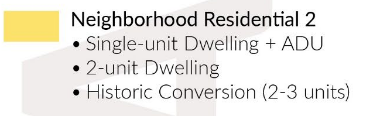
\includegraphics[width=0.3\textwidth,height=0.3\textheight,keepaspectratio]{resources/20240115/NR2.png}
\end{frame}

\begin{frame}{Placeholder}
    \begin{itemize}
        \item Put similar slides for the other two NR2 areas in South Medford here.
    \end{itemize}
\end{frame}

\begin{frame}{Overview of South Medford NR2}
    \centering
    \includegraphics[width=0.6\textwidth,height=0.6\textheight,keepaspectratio]{south_nr2.png}
    \hspace{0.5cm}
    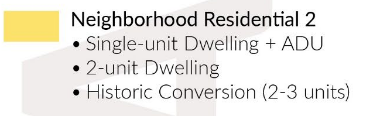
\includegraphics[width=0.3\textwidth,height=0.3\textheight,keepaspectratio]{resources/20240115/NR2.png}
\end{frame}

\begin{frame}{Additional Discussion}
    \begin{itemize}
    \item In the apartment-orientated NR districts, allow nonconforming single family homes to add an ADU. (Parcels might be too small to practically build a duplex, but detached garage to ADU conversion might be possible e.g.).
    \item Historical conversion should not primarily have a numerical unit limit. The limit should be based on size of the parcel or of the structure to be converted. 
    \item The City Council and the public do not have enough information about proposed historical conversion provisions to understand their impact on housing production.
    \item Is historical conversion going to be a niche opportunity for motivated and sophisticated developers on unicorn parcels? Or is this designed for average schmo to bring a lot of housing to the neighborhoods? 
    \end{itemize}
\end{frame}

\end{document}
